% 第 12 题四幅函数图的源图结构重绘；曲线高度与弯曲程度仅示意。
% 虚线 x=1 只出现在 f_2、f_3、f_4 面板，与固定 PDF 第 1 页一致。
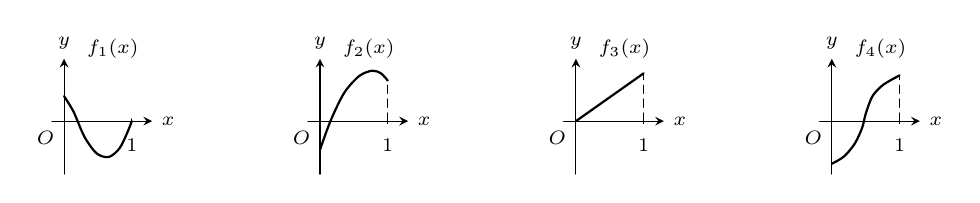
\begin{tikzpicture}[x=.86cm,y=.66cm,>=stealth,line cap=round,line join=round,
  every node/.style={font=\scriptsize}]
\foreach \shift/\name in {0/{f_1(x)},3.25/{f_2(x)},6.50/{f_3(x)},9.75/{f_4(x)}} {
  \begin{scope}[xshift=\shift cm]
    \draw[->] (-.18,0)--(1.30,0) node[right] {$x$};
    \draw[->] (0,-1.02)--(0,1.20) node[above] {$y$};
    \node[below left] at (0,0) {$O$};
    \draw (1,.045)--(1,-.045) node[below=2pt] {$1$};
    \node[above] at (.72,1.02) {$\name$};
  \end{scope}
}
% f_1：先降后升，右端在 x=1 处回到 x 轴；无辅助虚线。
\begin{scope}
  \draw[thick] plot[smooth] coordinates {
    (0,.48) (.14,.18) (.30,-.30) (.48,-.62) (.66,-.69)
    (.82,-.52) (.94,-.20) (1,0)
  };
\end{scope}
% f_2：从负值起始，凹向下上升并在 x=1 处收尾。
\begin{scope}[xshift=3.25cm]
  \draw[thick] plot[smooth] coordinates {
    (0,-.55) (.16,.02) (.36,.55) (.58,.87) (.77,.97) (.90,.92) (1,.78)
  };
  \draw[densely dashed] (1,0)--(1,.78);
\end{scope}
% f_3：从原点出发的线段，右端为 x=1。
\begin{scope}[xshift=6.50cm]
  \draw[thick] (0,0)--(1,.92);
  \draw[densely dashed] (1,0)--(1,.92);
\end{scope}
% f_4：下凸后上凸的 S 形曲线，穿过 x 轴后到达 x=1 端点。
\begin{scope}[xshift=9.75cm]
  \draw[thick] plot[smooth] coordinates {
    (0,-.82) (.18,-.68) (.34,-.43) (.45,-.12) (.50,.14)
    (.60,.48) (.76,.70) (1,.88)
  };
  \draw[densely dashed] (1,0)--(1,.88);
\end{scope}
\end{tikzpicture}
